\section{Does it matter when the agent drives?}
\label{sec:agent}

The probe holds the trajectory fixed and measures a distribution. The obvious
next question is whether any of it survives when the model chooses its own
actions, makes its own mistakes, and has several steps to recover from them.

\subsection{Setup}

Models act freely in ToolShed over \AgentNumTasks\ tasks, for up to
\AgentMaxSteps\ steps each, with greedy decoding. The task mix interleaves
single-call tasks (resolve a contact, write a file, set a reminder) with the two-
and three-call tasks used in the probe; without the easy tasks the smallest
models score zero under every harness and the comparison would be made on a
floor. A one-line format demonstration is appended to the system prompt,
identically in every condition. A task counts as solved only if the environment's goal predicate holds. There
is no partial credit and no model judges anything.

Two details of that demonstration are worth stating, because getting them wrong
cost us a full run. It shows the reply alone, with no speaker labels: an earlier
version presented a two-turn dialogue, and models copied the ``you:'' label into
their own replies, which the parser then rejected. The rate at which they did so
varied by harness, so a presentational choice had become a confound with the
comparison. Relatedly, the parser strips a leading speaker or action label
before parsing. That is the right behaviour independent of the bug: a harness
should not score a chat model's formatting habit as a tool-use failure. The
superseded rollouts are retained in the repository with an explanation rather
than deleted.

We compare \AgentNumHarnesses\ harnesses, which differ only in what the model
sees and in how its next token is chosen:
\emph{verbatim} (the standard transcript),
\emph{verbatim+instruction},
\emph{drop} (the failed step deleted, i.e.\ clean restart),
\emph{abstract} (failed calls replaced by a runtime-generated description),
\emph{verbatim+ban} (transcript unchanged, previously-failed strings blocked at
the decoder), and
\emph{abstract+ban}.

\subsection{Metrics}

Task success is the headline, but it is a coarse instrument at these model
sizes, so we report the mechanism alongside it.

\emph{Ended in a loop} is the fraction of rollouts that exhaust the step budget
having repeated an action. It is the outcome practitioners actually complain
about.

\emph{Exact repeat rate} is the fraction of failed actions that reproduce, byte
for byte, an action that already failed in the same rollout.

\emph{Canonical repeat rate} applies the same count after parsing the call and
sorting its keyword arguments, so a model that evades the ban by reordering
arguments or changing whitespace is still counted as repeating. That metric
exists to keep the ban honest: a decoder constraint trivially drives the exact
rate to zero, and the question is whether the model then does something useful
or merely paraphrases its mistake.

% Requires in the preamble:
% \newcommand{\ci}[2]{{\scriptsize\,[#1,\,#2]}}

\begin{table*}[t]
\centering
\small
\setlength{\tabcolsep}{4pt}
\begin{tabular}{l c c c}
\toprule
 & \multicolumn{3}{c}{Qwen2.5-0.5B} \\
Harness & success & exact rep. & canon. rep. \\
\midrule
verbatim (standard) & 0.42\,\ci{0.21}{0.62} & 0.31\,\ci{0.15}{0.47} & 0.31\,\ci{0.15}{0.47} \\
\quad + ``do not repeat'' & 0.58\,\ci{0.38}{0.79} & 0.24\,\ci{0.08}{0.42} & 0.24\,\ci{0.08}{0.42} \\
abstract & 0.33\,\ci{0.17}{0.54} & 0.16\,\ci{0.04}{0.31} & 0.16\,\ci{0.04}{0.31} \\
drop & 0.33\,\ci{0.17}{0.54} & 0.80\,\ci{0.79}{0.81} & 0.80\,\ci{0.79}{0.81} \\
verbatim + ban & 0.42\,\ci{0.21}{0.62} & 0.08\,\ci{0.00}{0.15} & 0.08\,\ci{0.00}{0.15} \\
abstract + ban & 0.33\,\ci{0.17}{0.54} & 0.07\,\ci{0.00}{0.14} & 0.07\,\ci{0.00}{0.14} \\
\bottomrule
\end{tabular}
\caption{End-to-end rollouts on ToolShed. Success is the environment's goal predicate; \emph{exact rep.} is the fraction of failed actions that repeat an earlier failed action byte for byte, and \emph{canon. rep.} applies the same count after parsing and normalising the call, so paraphrases of a banned string are still counted. Brackets give 95\% cluster bootstrap intervals over tasks.}
\label{tab:agent-main}
\end{table*}


\begin{figure*}[t]
\centering
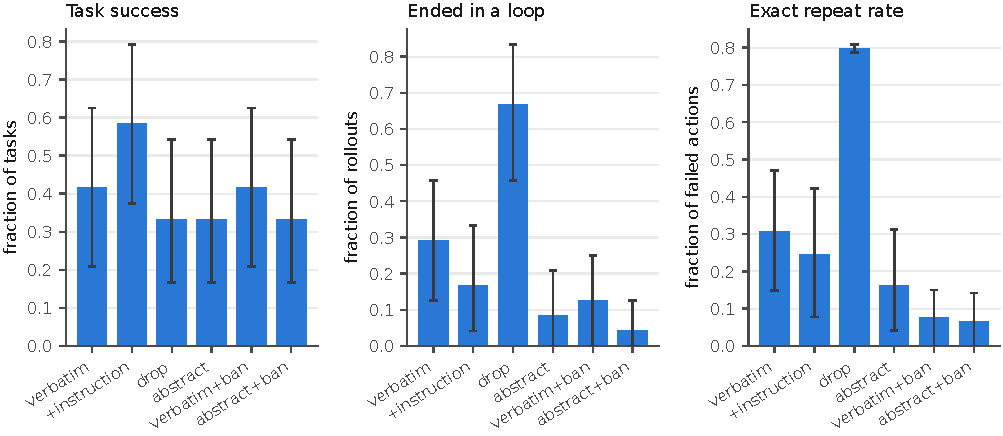
\includegraphics[width=0.9\linewidth]{figures/fig7_agent}
\caption{End-to-end rollouts, by harness. \textbf{Left:} task success.
\textbf{Middle:} the fraction of rollouts that end in a loop (step limit reached
with a repeated action). \textbf{Right:} the fraction of failed actions that
repeat an earlier failed action byte for byte. The two repetition panels order
the harnesses the same way, and it is the order the decomposition predicts:
interventions acting on the failed call's surface form at the good end, the
harness that deletes the failure outright at the bad end, the standard harness
in between. Task success does not follow that order, which
Section~\ref{sec:failure} explains. Error bars are 95\% cluster bootstrap
intervals over tasks.}
\label{fig:agent}
\end{figure*}

\subsection{Results}

\paragraph{The baseline behaves as the probe predicts.}
Under the standard harness the agent solves \AgentVerbatimSuccess\ of tasks, and
\AgentVerbatimRepeat\ of its failed actions are byte-for-byte repeats of an
action that already failed in the same rollout. Repetition is not a rare
pathology here; it is a substantial fraction of everything the agent does wrong.

\paragraph{Telling the model not to repeat does not reduce repetition, but it
does something else.}
Adding the prohibition to the system prompt moves the exact repeat rate by
\DeltaInstrRepeat\ points on matched tasks, an interval containing zero. The
probe reached the same verdict from a different direction
(Section~\ref{sec:analysis}): the instruction leaves the log-probability of
re-emitting the failed call essentially where it was, if anything nudging it the
wrong way.

Task success, however, moves by \DeltaInstrSuccess\ points, and that interval
excludes zero. The instruction also makes the agent \emph{cheaper}:
\AgentInstrTokens\ generated tokens per rollout against
\AgentVerbatimTokens, in fewer steps. We report this because it is what we
measured, and we decline to build a mechanism on it: with
\AgentNumTasks\ tasks the effect is real but the explanation is not identified,
and the most plausible readings, that the instruction makes the model more
careful in general or less willing to abandon a task early, are not about
repetition at all. The claim we do make is the narrow one the probe and the rollouts agree
on: a natural-language prohibition is not a repetition remedy.

\paragraph{Clearing the context is not a fix; it is the worst case.}
The remedy recommended by prior work on context contamination is to clear the
failed attempt before retrying \citep{yang2026contamination}. In our taxonomy
that is the \emph{drop} harness, and it is the harness that repeats most. The
exact repeat rate rises from \AgentVerbatimRepeat\ to \AgentDropRepeat, a
paired difference of \DeltaDropRepeat\ points whose interval is well clear of
zero, and task success does not improve (\DeltaDropSuccess).

The mechanism is worth stating plainly, because it reframes what the fix has to
be. Deleting the failed step restores the \emph{exact} context that produced the
failure. A deterministic policy in an identical context emits an identical action, so
clean restart does not remove the problem, it guarantees it. The
agent then spends its whole budget re-deriving the same call
(\AgentDropTokens\ generated tokens per rollout against
\AgentVerbatimTokens\ for the standard harness) and its rate of producing a
valid call falls.

This is specific to deterministic decoding, and we say so rather than
generalising it: with temperature sampling, resampling would supply the
variation the context no longer does. Greedy decoding is nonetheless a common
deployment choice, and the point survives in weaker form for any low-temperature
agent.

The three harnesses now form a clean design. \emph{verbatim} changes the context
using the failed string, which pulls the model back toward it. \emph{drop} does
not change the context at all, which leaves the model exactly where it was.
The requirement is therefore narrower than ``remove the failed action'':

\begin{quote}
The context after a failure must differ from the context before it, and the
difference must not be the failed action itself.
\end{quote}

\paragraph{Both surface-form interventions reduce repetition; the decoder ban
does so most cleanly.}
Blocking previously-failed strings at the decoder takes the exact repeat rate
from \AgentVerbatimRepeat\ to \AgentVerbBanRepeat, a paired difference of
\DeltaVerbBanRepeat\ points, with an interval clear of zero. The canonical rate
falls by the same amount, so the model is not paraphrasing its way around the constraint; it writes
genuinely different calls. Task success is
unchanged (\DeltaVerbBanSuccess), and the intervention costs no generated tokens
(\AgentVerbBanTokens\ against \AgentVerbatimTokens).

Replacing the call with a runtime-generated description does the same thing
through the context rather than the decoder, and lands between the ban and the
baseline: \AgentAbstractRepeat\ exact repeats, a paired difference of
\DeltaAbstractRepeat\ points whose interval touches zero at this sample size.

\paragraph{Neither surface-form intervention improves task success, and we say
so.}
The abstraction moves success by \DeltaAbstractSuccess\ points and the ban by
\DeltaVerbBanSuccess. This is the result we would most like to have come out
otherwise, and it is worth being direct about what it does and does not
undermine.

The interventions were derived from a mechanism. They move that mechanism, by
roughly the predicted amount and in the predicted direction, and the harness
that our decomposition says should be worst is indeed dramatically worst. What they do not do is convert that into task success at this scale, which
Section~\ref{sec:failure} explains: \ProseShare\ of this model's actions are
prose where a call was expected, a failure no arrangement of the transcript
repairs. Removing the loop returns the agent's budget to it; whether it can
spend that budget well is a question about the model, not the harness.

The instruction is the instructive contrast. It raises success
(\DeltaInstrSuccess\ points) while leaving repetition where it was; the
surface-form interventions do the reverse. They act on different things. Only
the second kind is evidence about the mechanism this paper is concerned with,
and a practitioner who wants task success from a 0.5B agent should not expect
either to be the whole answer.

\paragraph{The ban stops the loop but does not solve the task.}
Applying the decoder ban to the unmodified transcript cuts exact repetition to
near nothing (\DeltaVerbBanRepeat\ points, from \AgentVerbatimRepeat\ to
\AgentVerbBanRepeat) and eliminates loops
(\AgentVerbBanStuck\ of rollouts against \AgentVerbatimStuck), at a cost of
\AgentVerbBanTokens\ generated tokens per rollout against
\AgentVerbatimTokens. Task success does not move at all
(\DeltaVerbBanSuccess).

That combination is worth dwelling on, because it separates two things the
paper could otherwise be read as conflating. The canonical repeat rate equals
the exact rate in every harness we ran, to the digit, so the residual
repetition is not the model paraphrasing its way around the constraint. It is
the ban's own boundary: the mask is over token sequences in the raw generation,
while a repeat is counted over the parsed action, and the two come apart when
the generation is cut off by the token cap or when the same visible string is
reached by a different token path. Inspecting the three rollouts (of
\AgentNumTasks) in which any exact repeat survives the ban, the repeated string is in every case one the parser rejected, either
unterminated prose or a call with an unbalanced parenthesis, and never a
well-formed call. Forbidding a string
prevents the agent from wasting its budget, and nothing more. Removing the
string from the context lets the agent reconsider.

\paragraph{The two interventions are complementary, not redundant.}
Applying the ban on top of the abstraction reduces exact repetition further,
from \AgentAbstractRepeat\ to \AgentAbsBanRepeat\ (\DeltaAbsBanRepeat\ points
against the standard harness, an interval clear of zero where the abstraction
alone is not). The instrumentation says why: under the abstracted transcript the
ban still fires, on roughly half as many decoding steps as it does under the
verbatim transcript, but far from never.

That is worth stating because it refines the mechanism. Removing the failed
call from the context removes the model's opportunity to \emph{copy} it, but
not its ability to \emph{re-derive} it: the goal, the tool schemas and the
successful prefix are all still there, and they are what produced the wrong call
in the first place. The context edit and the decoder constraint therefore catch different things,
one the copying and the other the residue, and a harness that wants neither
should do both. Neither costs a generated token.

\paragraph{Summary of the ordering.}
Ranked by the fraction of rollouts that end in a loop: abstract+ban
(\AgentAbsBanStuck), abstract (\AgentAbstractStuck) and verbatim+ban
(\AgentVerbBanStuck) at the good end; the ``do not repeat'' instruction at
\AgentInstrStuck; the standard harness at \AgentVerbatimStuck; and clean
restart worst at \AgentDropStuck. Ranking by exact repeat rate gives the same
order. Interventions that act on the failed call's surface form occupy the good
end, the harness that deletes the failure outright occupies the bad end, and the standard harness sits between. That is the ordering the decomposition
predicts, arrived at without reference to it.

Task success does not follow that ordering, and we would rather flag the
mismatch than bury it. The best harness for success is the one that does least
about repetition. Section~
ef{sec:failure} gives the reconciliation: at this
scale repetition is a large share of what goes wrong but not the largest, and an
intervention that removes it cannot remove the rest.

\subsection{Does the probe agree with the rollouts?}

Within this model the two studies agree on every comparison they both make. The
probe says the abstraction removes almost all of the inversion and drives the
exact greedy repeat rate to zero; the rollouts show the same, and add that task
success rises. The probe says the natural-language prohibition does not help
(\DInstructionCI\ nats, slightly the wrong way); the rollouts show it increasing
exact repetition. The probe's clean-restart baseline is the \emph{pre}
condition by construction, and the rollouts show why restoring that context is
not a remedy.

What we cannot yet do is test whether the probe \emph{predicts across models},
that is, whether a model with a more negative $\Gain$ loops more in practice. That needs
rollouts for several models, and rollouts are three orders of magnitude more
expensive than probe items on the hardware available here (Section~\ref{sec:efficiency}).
It is the experiment we would run first with a GPU, and it is the one that would
turn the probe from an explanation into a cheap diagnostic: a harness designer
could then measure $\Gain$ on a few hundred items rather than running a full
agent evaluation.
